\documentclass[dvisvgm,multi=true]{standalone}
\usepackage{mathmlcoresvg}
\begin{document}
%<figcaption><span>Figure 10: </span>Box model for the <code>mfrac</code> element without bar</figcaption>
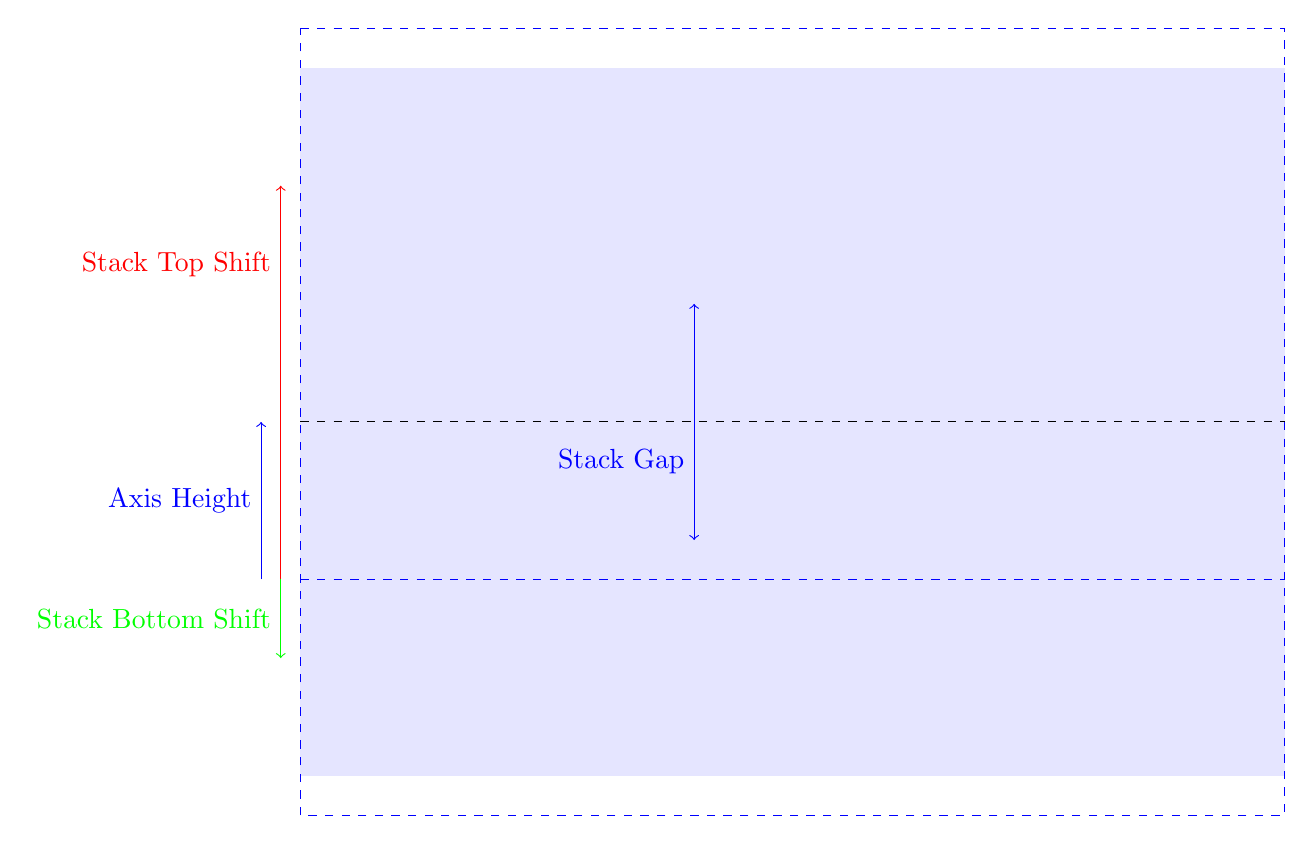
\begin{tikzpicture}[yscale=-1]
  \fill[blue!10] (0,-6.5) -- (12.5,-6.5) -- (12.5,2.5) -- (0,2.5) -- cycle;
  \MathMLBox{0}{-5}{2.5}{1}{red}
  \MathMLBox{3.75}{1}{1}{1}{green}
  \draw[dashed,blue] (0,-7) -- (12.5,-7) -- (12.5,3) -- (0,3) -- cycle
  (0,0) -- (12.5,0);
  \draw[black,dashed] (0,-2) -- (12.5,-2);
  \draw[->,blue] (-.5,0) -- (-.5,-1) node[left]{Axis Height} -- (-.5,-2);
  \draw[->,red] (-.25,0) -- (-.25,-4)
  node[left]{Stack Top Shift} -- (-.25,-5);
  \draw[->,green] (-.25,0) -- (-.25,.5)
  node[left]{Stack Bottom Shift} -- (-.25,1);
  \draw[<->,blue] (5,-3.5) -- (5,-1.5) node[left]{Stack Gap} --
  (5,-.5);
\end{tikzpicture}

\end{document}
